\documentclass[journal]{IEEEtran}
\usepackage[a5paper, margin=10mm, onecolumn]{geometry}
\usepackage{tfrupee}
\usepackage{gvv-book}
\usepackage{gvv}
\usepackage{cite}
\usepackage{amsmath,amssymb,amsfonts,amsthm}
\usepackage{algorithmic}
\usepackage{graphicx}
\usepackage{textcomp}
\usepackage{xcolor}
\usepackage{txfonts}
\usepackage{listings}
\usepackage{enumitem}
\usepackage{mathtools}
\usepackage{gensymb}
\usepackage{comment}
\usepackage[breaklinks=true]{hyperref}
\usepackage{tkz-euclide}
\usepackage{listings}
\def\inputGnumericTable{}
\usepackage[latin1]{inputenc}
\usepackage{color}
\usepackage{array}
\usepackage{longtable}
\usepackage{calc}
\usepackage{multirow}
\usepackage{hhline}
\usepackage{ifthen}
\usepackage{lscape}
\begin{document}
	
	\bibliographystyle{IEEEtran}
	\vspace{3cm}
	
	\title{11.16.4.3.3}
	\author{EE24BTECH11022 - ESHAN SHAMRMA}
	\maketitle
	\textbf{Question:}
	A die has two faces each with number '1', three faces each with number '2', and one face with number '3'. If the die is rolled once, determine the probability of not rolling a '3', i.e., \( P(X \neq 3) \).
	
	\textbf{Solution:}
	
	\textbf{Step 1: Define the Probability Mass Function (PMF)}
	
	Let the random variable \( X \) represent the outcome of rolling the given die. The die has:
	- 2 faces with number \( 1 \),
	- 3 faces with number \( 2 \),
	- 1 face with number \( 3 \).
	
	The total number of faces on the die is:
	\[
	N = 2 + 3 + 1 = 6.
	\]
	
	Thus, the probability mass function (PMF) \( p_X(n) \) is given by:
	\[
	p_X(n) = P(X = n) = \frac{\text{number of faces with } n}{\text{total number of faces}}.
	\]
	
	Using this definition, we obtain:
	\[
	p_X(n) =
	\begin{cases}
		\frac{2}{6} = \frac{1}{3}, & n = 1, \\
		\frac{3}{6} = \frac{1}{2}, & n = 2, \\
		\frac{1}{6}, & n = 3, \\
		0, & \text{otherwise}.
	\end{cases}
	\]
	
	\textbf{Step 2: Compute the Cumulative Distribution Function (CDF)}
	
	The cumulative distribution function (CDF) \( F_X(n) \) is given by:
	\[
	F_X(n) = P(X \leq n) = \sum_{k \leq n} p_X(k).
	\]
	
	Computing for different values of \( n \):
	\[
	F_X(n) =
	\begin{cases}
		0, & n < 1, \\
		P(X = 1) = \frac{1}{3}, & 1 \leq n < 2, \\
		P(X = 1) + P(X = 2) = \frac{1}{3} + \frac{1}{2} = \frac{5}{6}, & 2 \leq n < 3, \\
		1, & n \geq 3.
	\end{cases}
	\]
	
	\textbf{Step 3: Compute the Probability of Not Rolling a '3'}
	
	The event "not rolling a 3" corresponds to \( X \leq 2 \), i.e., \( P(X \neq 3) = P(X = 1) + P(X = 2) \). Using our PMF:
	\[
	P(X \neq 3) = P(X = 1) + P(X = 2) = \frac{1}{3} + \frac{1}{2}.
	\]
	
	Converting to a common denominator:
	\[
	P(X \neq 3) = \frac{2}{6} + \frac{3}{6} = \frac{5}{6}.
	\]
	
	Alternatively, using the CDF:
	\[
	P(X \neq 3) = P(X \leq 2) = F_X(2) = \frac{5}{6}.
	\]
	
	\textbf{Final Answer:}
	\[P(X \neq 3) = \frac{5}{6}.\]
	
	
	\textbf{Simulation:}
	To verify the probability \( P(\text{not } 3) \), we can simulate rolling the die multiple times and compute the empirical probability. Below are the plots for the simulation:
	
	\begin{figure}[h]
	\centering
	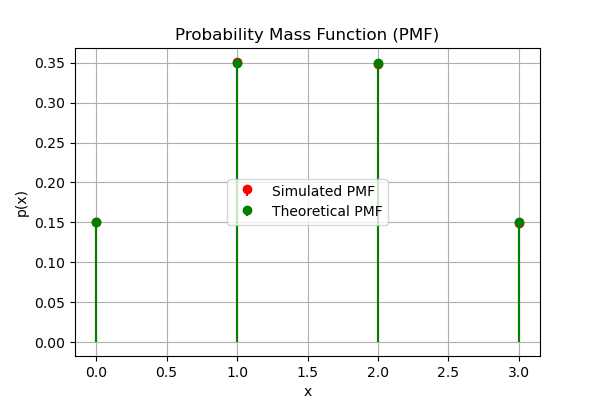
\includegraphics[width=0.8\textwidth]{figs/pmf.png}
	\end{figure}
	
	\begin{figure}[h]
		\centering
		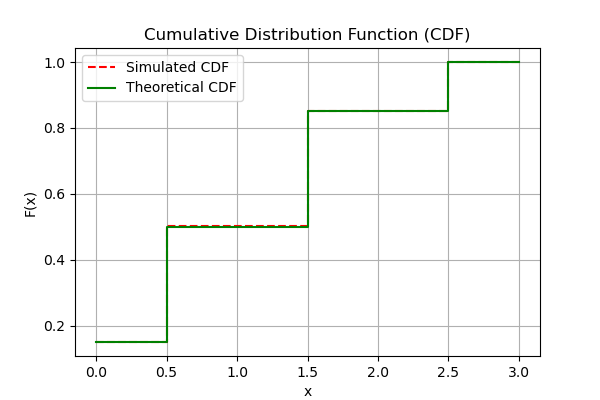
\includegraphics[width=0.8\textwidth]{figs/cdf.png}
	\end{figure}
	
\end{document}